\section{Implementation}
{\tiny Written by: Philipp Becker}
\subsection{Frontend} \label{sec:Frontend_Implementation}
This subsection provides an overview of the implementation details for the front end of the locker system. It deals with the technologies, frameworks and development environment in use during the development process.

\subsection{Frontend Implementation}
\subsubsection{Project Setup}

The frontend of our locker system utilizes Vue.js, equipped with auxiliary libraries such as Vue Router for routing,  BootstrapVue3 for interface design, chosen for their robustness and effective integration capabilities.

\paragraph{Development Environment Preparation}
To set up the development environment, Node.js is required for utilizing npm, which manages the project's dependencies. The project is cloned from its GitHub repository, which includes essential configuration files such as \texttt{package.json}. The repository may contain additional configuration files like \texttt{.gitignore}, \texttt{.eslintrc.json}, \texttt{.prettierrc}, and \texttt{README.md}. These files help configure version control, code linting, formatting, and provide project documentation, respectively.



\paragraph{Dependencies and Local Server}
In the project directory, dependencies are installed via \texttt{npm install}, incorporating Vue Router and BootstrapVue3. The local development server is initiated with \texttt{npm run dev}, providing a live-reload feature beneficial during development.

\paragraph{Configuration and Build}
Environment variables are configured to manage API endpoints effectively. The \texttt{npm run build} command compiles the application into a 'dist' folder, segmenting it into optimized chunks that improve load efficiency, ideal for deployment.

\paragraph{Quality Assurance}
Integration of ESLint and Prettier ensures code quality and consistency, essential for maintaining high standards in collaborative development environments.

This setup process outlines a systematic approach to preparing a scalable and efficient development environment for the Vue.js frontend, aligned with contemporary web development best practices.

\subsubsection{Project Structure}

This section outlines the structural framework of the Vue.js application, focusing on the core components that define its architecture. A well-organized project structure is crucial for efficient development and maintenance.

\begin{itemize}
    \item \textbf{README.md}: This file serves as the project's main documentation hub, containing comprehensive information on setup instructions, deployment steps, and other essential details. A well-written README enhances project understanding and facilitates collaboration among team members.

    \item \textbf{Main.ts}: The entry point for the Vue application. This file initializes the root Vue instance, sets up the initial plugins, dependencies, and mounting point for the app to the DOM.

    \item \textbf{App.vue}: The main Vue component that acts as the root of the application. It integrates the primary structure or layout and serves as the entry point for the component hierarchy.

    \item \textbf{components}: This directory houses reusable Vue components that can be utilized across different parts of the application, such as buttons, input fields, and dialogs, helping to maintain a clean and modular structure.

    \item \textbf{views}: Contains Vue components that represent different pages or routes of the application. These are typically larger and more complex than simple components and form the main parts of the application interface.

    \item \textbf{router}: Manages the routing configuration for the application. It defines the routes and their corresponding components, enabling navigation between different views within the application.

    \item \textbf{assets}: This directory stores static resources such as images, stylesheets, and fonts that are used by the application. It helps in organizing and managing the UI resources that are not part of Vue component logic.
\end{itemize}

\subsubsection{Vue.js Imports and Mounting}
\begin{itemize}
    \item \textbf{Imports and Styles Configuration:} The Main.ts file plays a crucial role in setting up the Vue.js application by importing essential libraries and styles. It includes the Vue framework, the main component App.vue, the router, and Pinia for state management. For the user interface, BootstrapVue3 and Bootstrap icons are imported along with their respective CSS files to ensure the application is both functional and aesthetically pleasing.
    \begin{lstlisting}[language=TypeScript]
import { createApp } from 'vue';
import App from './App.vue';
import router from './router';
import BootstrapVue3 from 'bootstrap-vue-3';
import { BootstrapIconsPlugin } from "bootstrap-icons-vue";
import './css/index.css';
import 'bootstrap/dist/css/bootstrap.css';
import 'bootstrap-vue-3/dist/bootstrap-vue-3.css';
    \end{lstlisting}

    \item \textbf{Application Setup and Mounting:} After importing the necessary modules, the application is instantiated and configured in Main.ts. Key steps include setting global properties like the backend link, and integrating BootstrapVue3, Bootstrap icons and the router. The application is then mounted to the DOM at the 'app' selector, initializing the system's frontend.
    \begin{lstlisting}[language=TypeScript]
const app = createApp(App)
app.config.globalProperties.backendLink = 'https://f-itplfo6nya-uc.a.run.app'
app.use(BootstrapVue3)
app.use(BootstrapIconsPlugin)
app.use(router)
app.mount('#app')
    \end{lstlisting}
\end{itemize}
\subsubsection{Vue.js-File Introduction}
In vue.js, individual vue files are divided into three parts. These start with a template part, followed by a script part and optionally a style part can be created.
The HTML code is written in the template part. However, libraries such as BootstrapVue can also be used in this part to use ready-made HTML elements. In the script part, the page is initialized and all functions that this special page uses can be defined. Comprehensive functions are integrated in the import of the script part. If it is necessary to style HTML elements differently on a specific page, a style section can be added in which CSS classes can be defined.
\begin{itemize}
\item \textbf{template:}
\begin{lstlisting}[language=HTML]
<template>
  <div class="mx-auto my-10" style="width: 90%;">
    <h3 class="text-left">Admin Dashboard</h3>
    <dashboard-charts></dashboard-charts>
    <div class="d-flex justify-content-center align-items-center pt-10">
      <iframe width="450" height="260" style="border: 1px solid #cccccc;" src="https://thingspeak.com/channels/2530450/widgets/852176"></iframe>

      <iframe width="450" height="260" style="border: 1px solid #cccccc;" src="https://thingspeak.com/channels/2530450/charts/1?bgcolor=%23ffffff&color=%23d62020&dynamic=true&results=60&title=History+of+Wattage&type=line"></iframe>
    </div>

    <div class="flex justify mt-4">
    </div>
  </div>
</template>
    \end{lstlisting}

\item \textbf{script:}
\begin{lstlisting}[language=TypeScript]
<script lang="ts">
import { defineComponent } from 'vue';
import DashboardCharts from '@/components/DashboardCharts.vue';

export default defineComponent({
  components: {
    DashboardCharts,
  },
  setup() {

    return {
    }
  },
})
</script>
    \end{lstlisting}
\item \textbf{style:}
\begin{lstlisting}[language=TypeScript]
</script>
<style>
.pin-container {
  display: flex;
  justify-content: center;
  font-family: Arial, sans-serif;
</style>
    \end{lstlisting}
\end{itemize}

\subsubsection{Vue Components}
vue components can be created as .vue files and can therefore be imported and used on any vue screen. The following example shows our footer, which is then integrated into the template part of a sample vue.
\begin{itemize}
  \item \textbf{Creating of Component}

\begin{lstlisting}[language=HTML]
<template>
  <footer class="footer bg-light text-center text-lg-start">
    <div class="container p-4">
      <div class="row">
        <div class="col-lg-6 col-md-12 mb-4 mb-md-0">
          <h5 class="text-uppercase">Database Inventory Locker System</h5>
          <p>We provide your favorite Tools for rent.</p>
          <p>Your Devices are safe and charged after storing.</p>
        </div>
        <div class="col-lg-6 col-md-12 mb-4 mb-md-0 text-lg-end">
          <h5 class="text-uppercase">Follow Us on Social Media</h5>
          <p>
            <span class="p-2" style="font-size: 24px;">Icon1</span>
            <span class="p-2" style="font-size: 24px;">Icon2</span>
          </p>
        </div>
      </div>
    </div>

    <div class="text-center p-3" style="background-color: rgba(0, 0, 0, 0.05);">
    2024
      <a class="text-dark" href="https://databaseinventorysystem.com/">databaseinventory.com</a>
    </div>
  </footer>
</template>

    \end{lstlisting}
\item \textbf{Usage of the Component}
    \begin{lstlisting}[language=HTML]
<template>
  <Footer_component></footer_component>
</template>
#Import 
<script>
import Footer_component from "@/components/footer_component.vue";
</script>
    \end{lstlisting}
\end{itemize}
\subsubsection{Implementing Role-Based Access Control}
The useLoggedIn composable encapsulates the management of user authentication states within a Vue.js application, utilizing Vue's reactive system. This composable serves as a centralized mechanism to manage and react to changes in the user's login status, which is pivotal in implementing role-based access controls (RBAC). Below, the functionality and internal mechanisms of the useLoggedIn composable are dissected and explained:

\begin{itemize}
\item \textbf{Composition Function}
The useLoggedIn function exports a reactive reference, loggedIn, initialized to "None", indicating no user is currently authenticated. The function returns an object containing this reactive state alongside functions setLoggedIn and checkLoggedIn, which manipulate and assess the authentication state, respectively.
\begin{lstlisting}[language=TypeScript]
import { type Ref, ref } from "vue";
export type LoggedIn = "Admin" | "User" | "None";
const loggedIn: Ref<LoggedIn> = ref("None");
export const useLoggedIn = () => {
    return {
        loggedIn,
        setLoggedIn,
        checkLoggedIn,
    };
}
\end{lstlisting}
\item \textbf{Check Login Status}
The checkLoggedIn method evaluates the user's role by reading the sessionStorage where the user's role is persisted across sessions. Depending on the stored value, it sets the loggedIn state to "Admin", "User", or "None", effectively updating the authentication status based on session data.

\begin{lstlisting}[language=TypeScript]
const checkLoggedIn = () => {
    if (sessionStorage.getItem("isAdmin") === "true") {
        loggedIn.value = "Admin";
    } else if (sessionStorage.getItem("isAdmin") === "false") {
        loggedIn.value = "User";
    } else {
        loggedIn.value = "None";
    }
};
\end{lstlisting}
\item \textbf{Set Login Status}
The setLoggedIn function is used to explicitly set the authentication status. It updates the sessionStorage to reflect the new role ("Admin" or "User") or clears it if logging out. This method also updates the reactive loggedIn state, triggering any dependent components to re-render based on the new authentication status.

\begin{lstlisting}[language=TypeScript]
const setLoggedIn = (l: LoggedIn) => {
    console.log(l);
    if (l == "Admin") {
        sessionStorage.setItem("isAdmin", "true");
    } else if (l == "User") {
        sessionStorage.setItem("isAdmin", "false");
    }
    else{
        sessionStorage.removeItem('isAdmin');
    }
    loggedIn.value = l;
};
\end{lstlisting}
\end{itemize}

\subsubsection{Sitemap Overview}
This section presents the sitemaps for both the Admin and User frontends of the Invetory Managment System. These sitemaps are visual representations that detail the structure and navigational schema of the respective interfaces. By examining these sitemaps, one can gain a comprehensive understanding of the user flow and interaction design implemented in both the administrative and user-facing sections of the application.
\begin{itemize}
\item \textbf {Admin Frontend}
\begin{figure}[h]
    \centering
    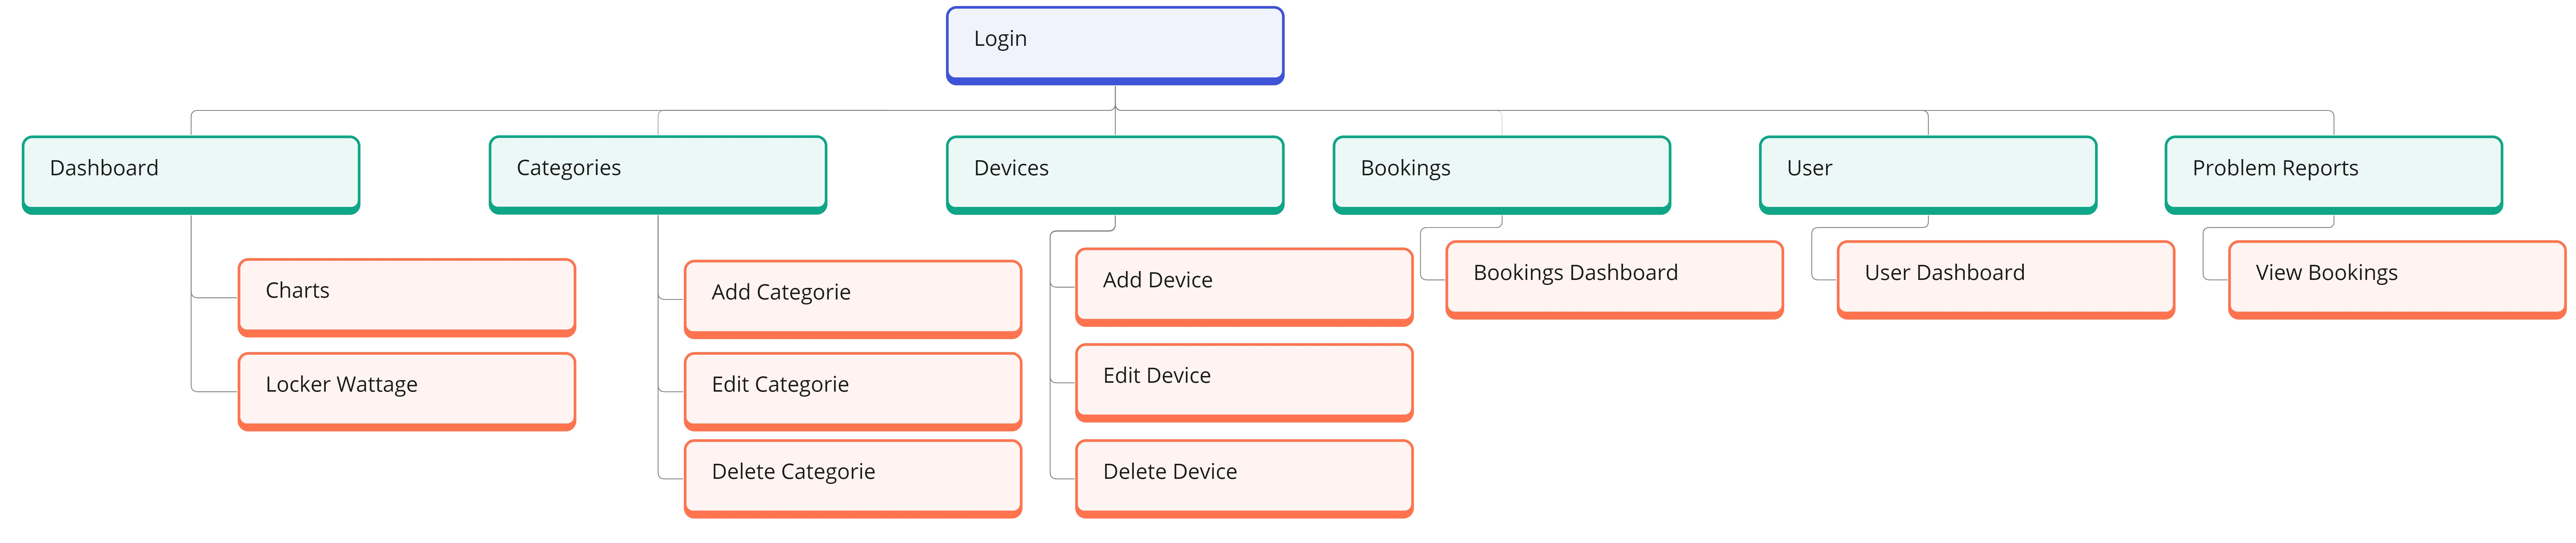
\includegraphics[width=1\textwidth]{images/Sitemap.jpg}
    \caption{Admin Frontend Sitemap}
    \label{fig:myimage}
\end{figure}
\clearpage
\item \textbf {User Frontend}
\begin{figure}[h]
    \centering
    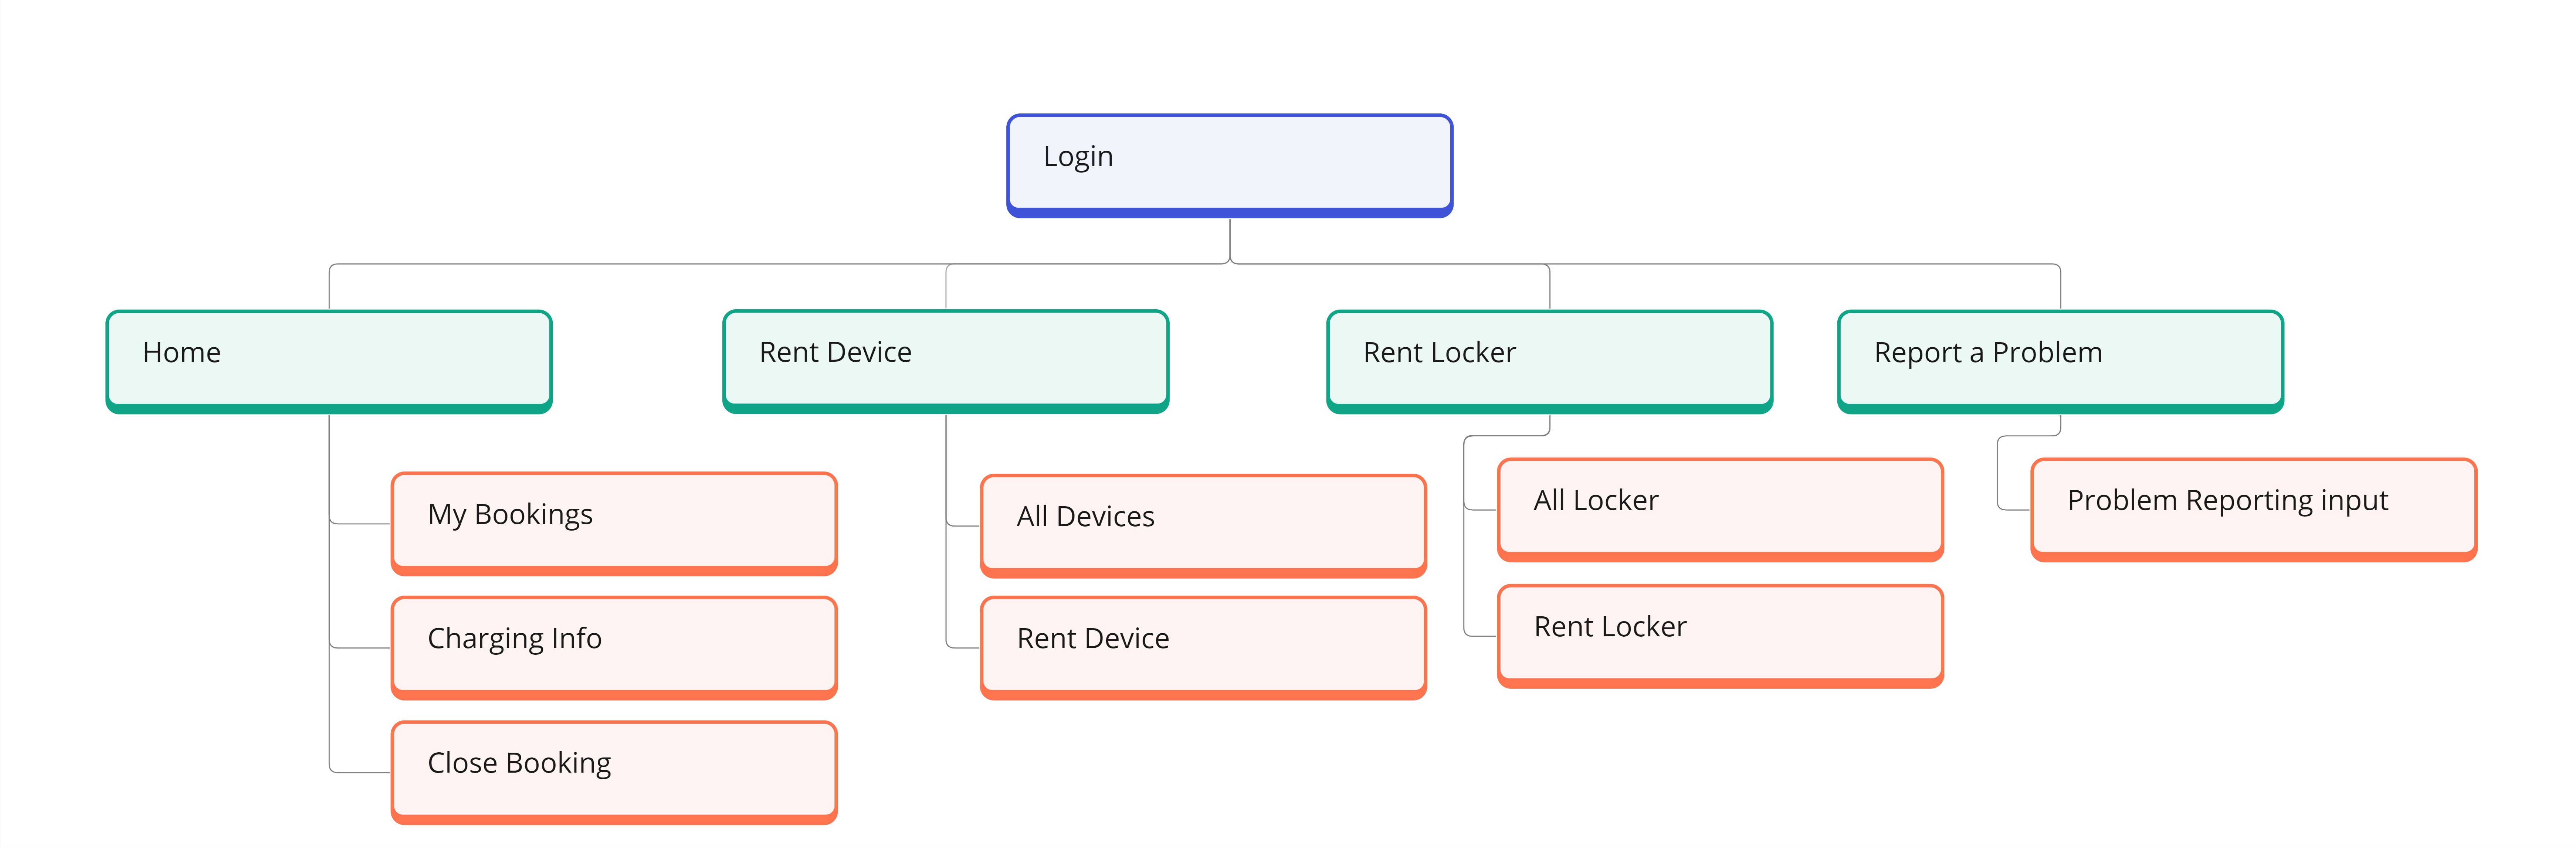
\includegraphics[width=1\textwidth]{images/usersitemap.jpg}
    \caption{User Frontend Sitemap}
    \label{fig:myimage}
\end{figure}
\end{itemize}

\subsubsection{Frontend Demo Screenshots}
This section provides a visual demonstration of the frontend interface, starting with the Admin-Portal Dashboard. 
\begin{itemize}
\item \textbf {Admin Dashboard: } The dashboard offers a comprehensive overview of all device bookings and displays revenue statistics for recent months. Our safety intentions are to monitor the current flow in each locker, so we have opted for the following overview: The dashboard includes a overview for current wattage and a wattage history for booked lockers.
\begin{figure}[h]
    \centering
    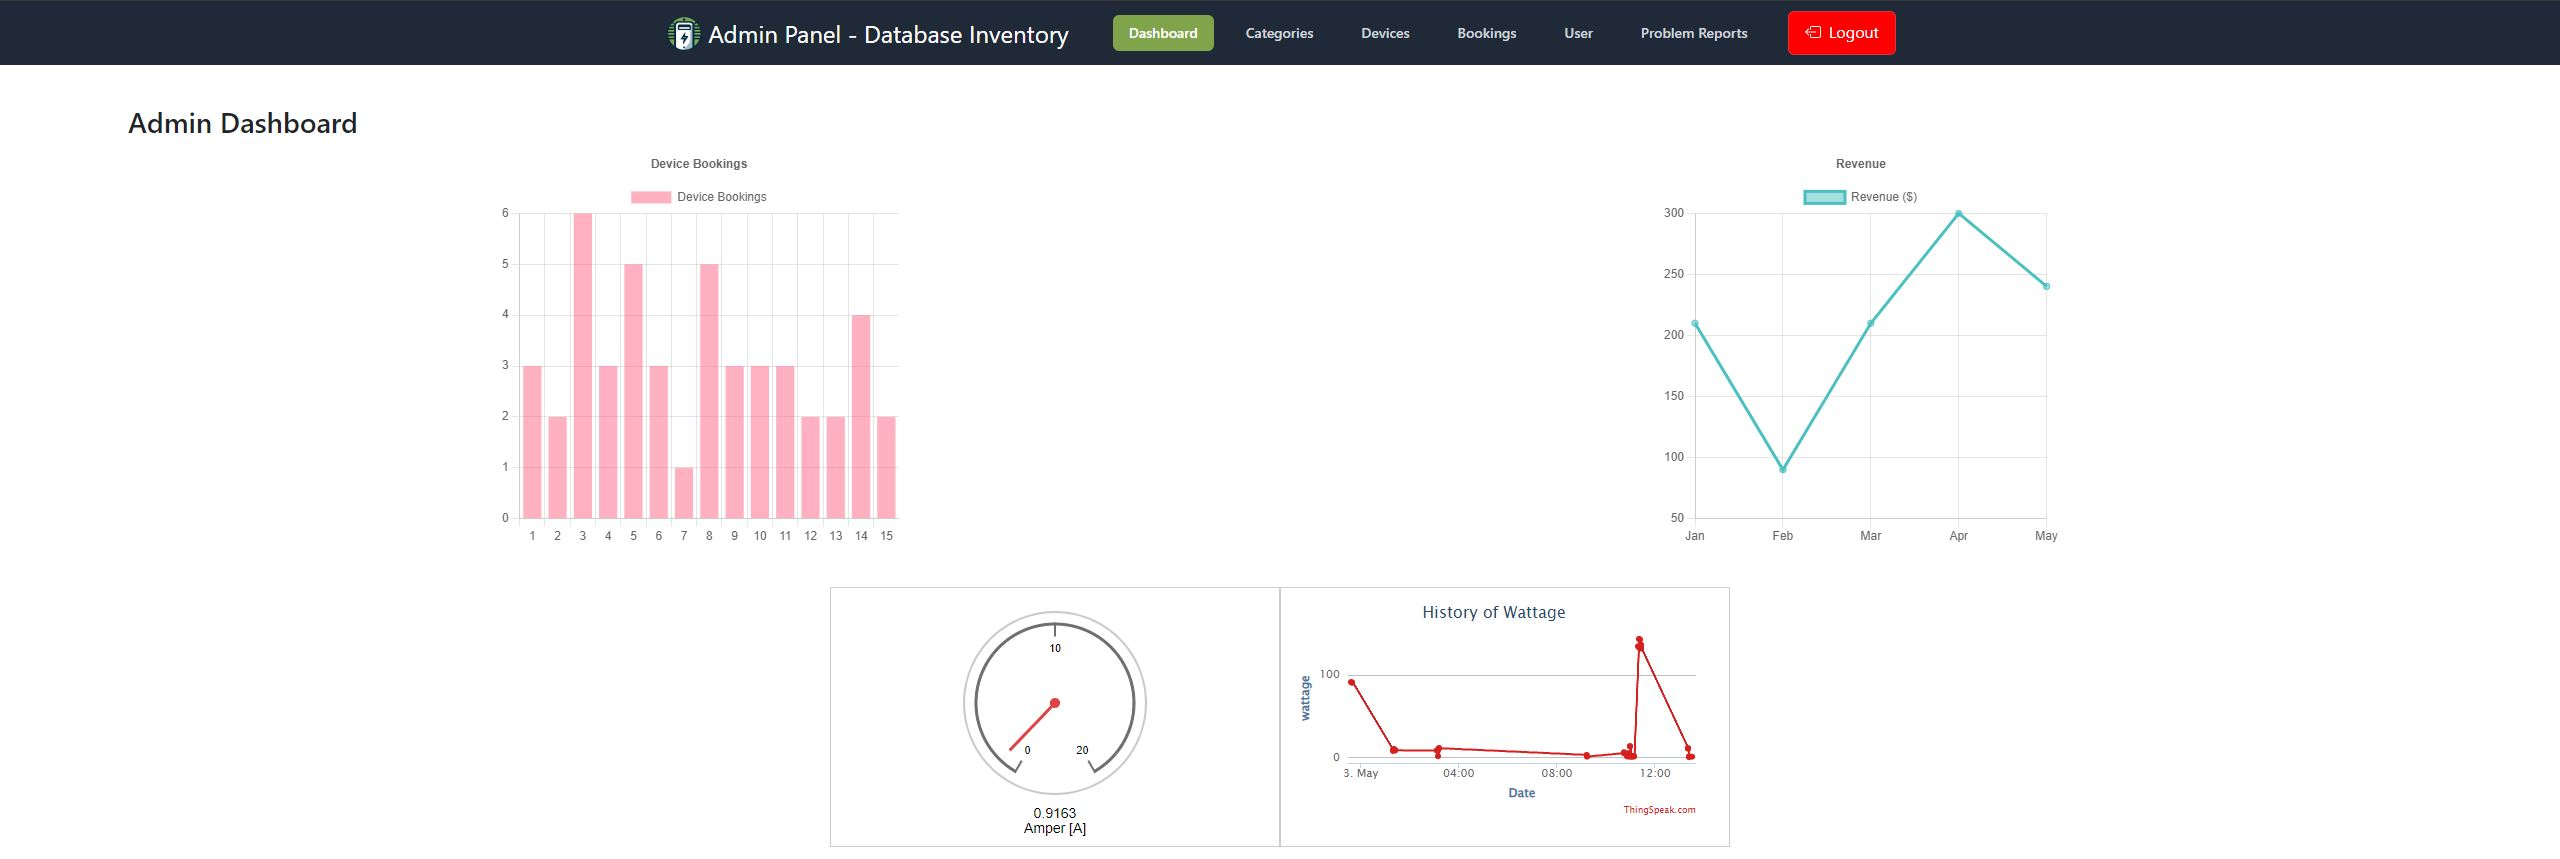
\includegraphics[width=1\linewidth]{images/admin-dashboard.JPG}
    \caption{Admin Dashboard}
    \label{fig:admin-dashboard}
\end{figure}

\item \textbf {Categories Screen: }In the Categories Screen, administrators can view all categories that have been added to the Inventory Management System. Each category can be edited or deleted, and new categories can be added, providing flexible management of the system's categorization logic.
\begin{figure}[h]
    \centering
    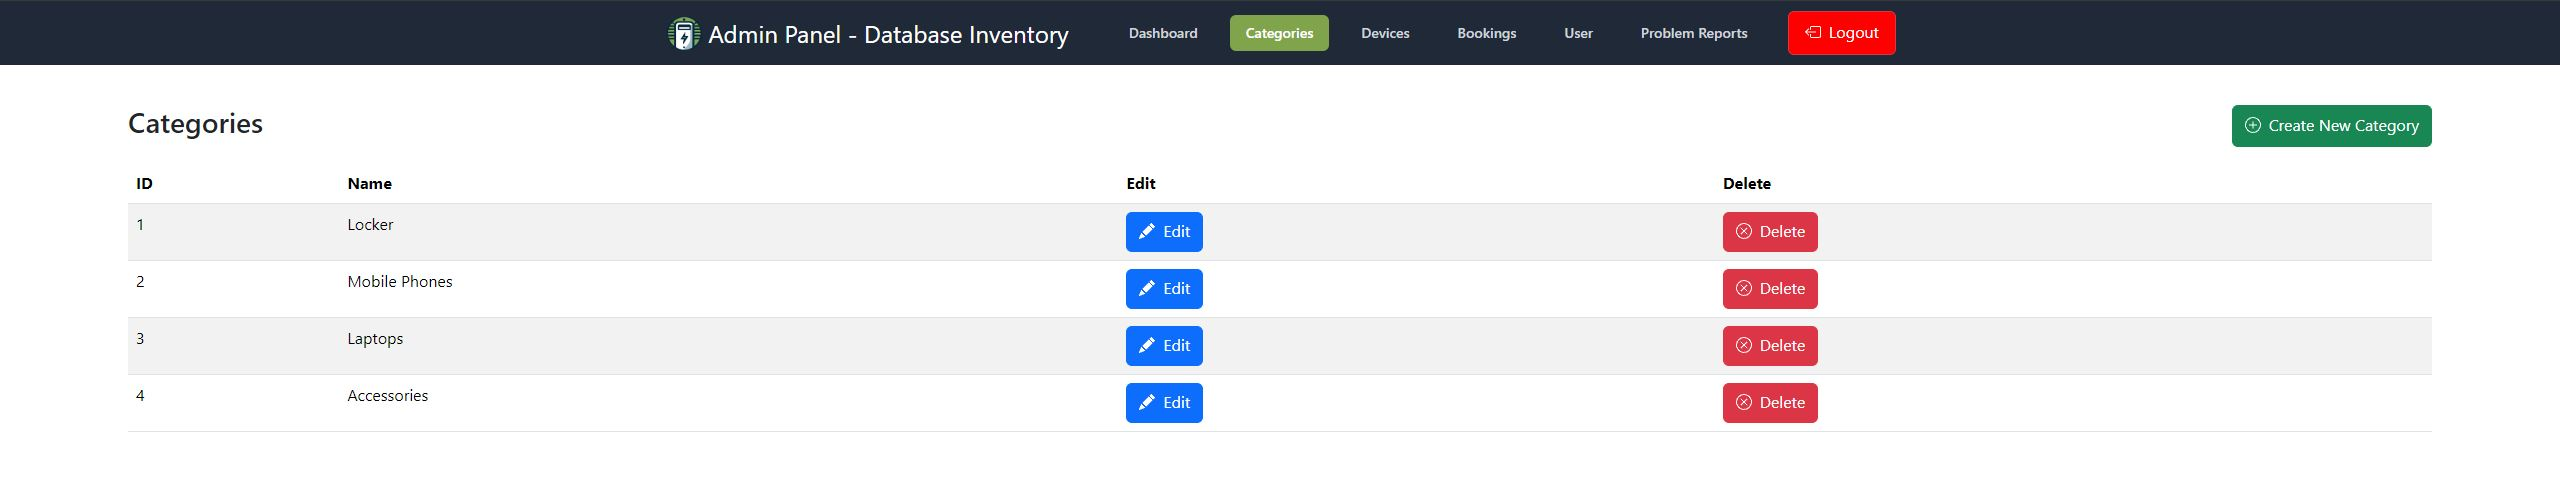
\includegraphics[width=1\linewidth]{images/categories.JPG}
    \caption{Admin Dashboard Categories}
    \label{fig:categories-dashboard}
\end{figure}


\item \textbf {Edit Categories Screen: }This figure depicts the Edit Category Modal, where administrators can easily modify the name of a category, enhancing the adaptability of system configurations.
\begin{figure}[h]
    \centering
    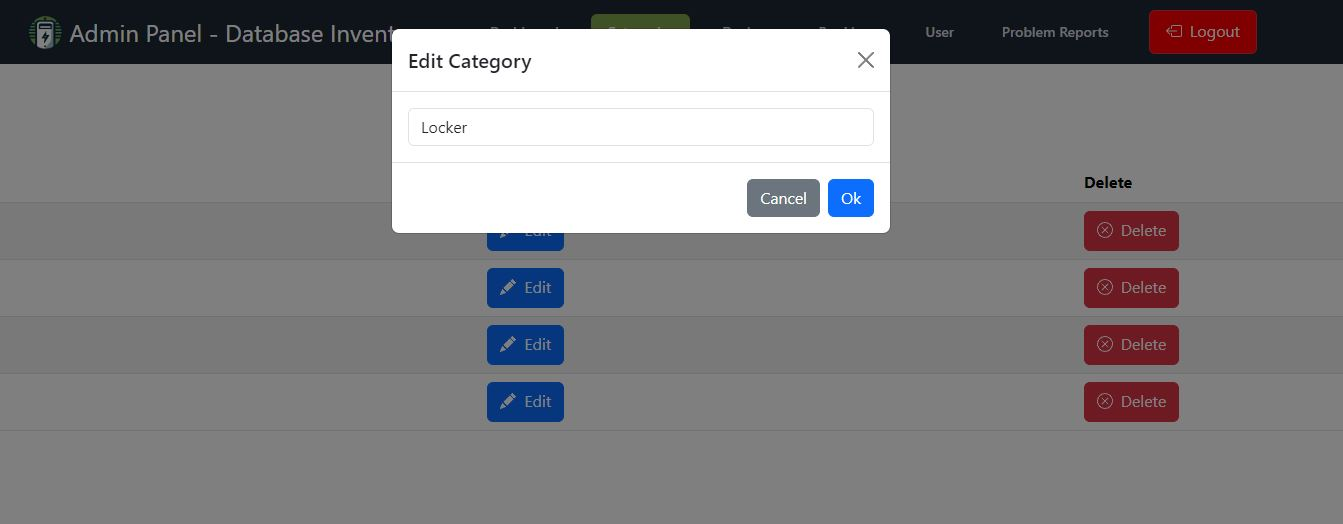
\includegraphics[width=1\linewidth]{images/edit categorie.JPG}
    \caption{Admin Dashboard Edit Categories Modal}
    \label{fig:edit-category-modal}
\end{figure}


\item \textbf {Devices Screen: }The Devices Screen displays all devices that have been integrated into the system. This interface allows for the addition of new items and the modification of existing devices, ensuring that the system remains up-to-date and functional.
\begin{figure}[h]
    \centering
    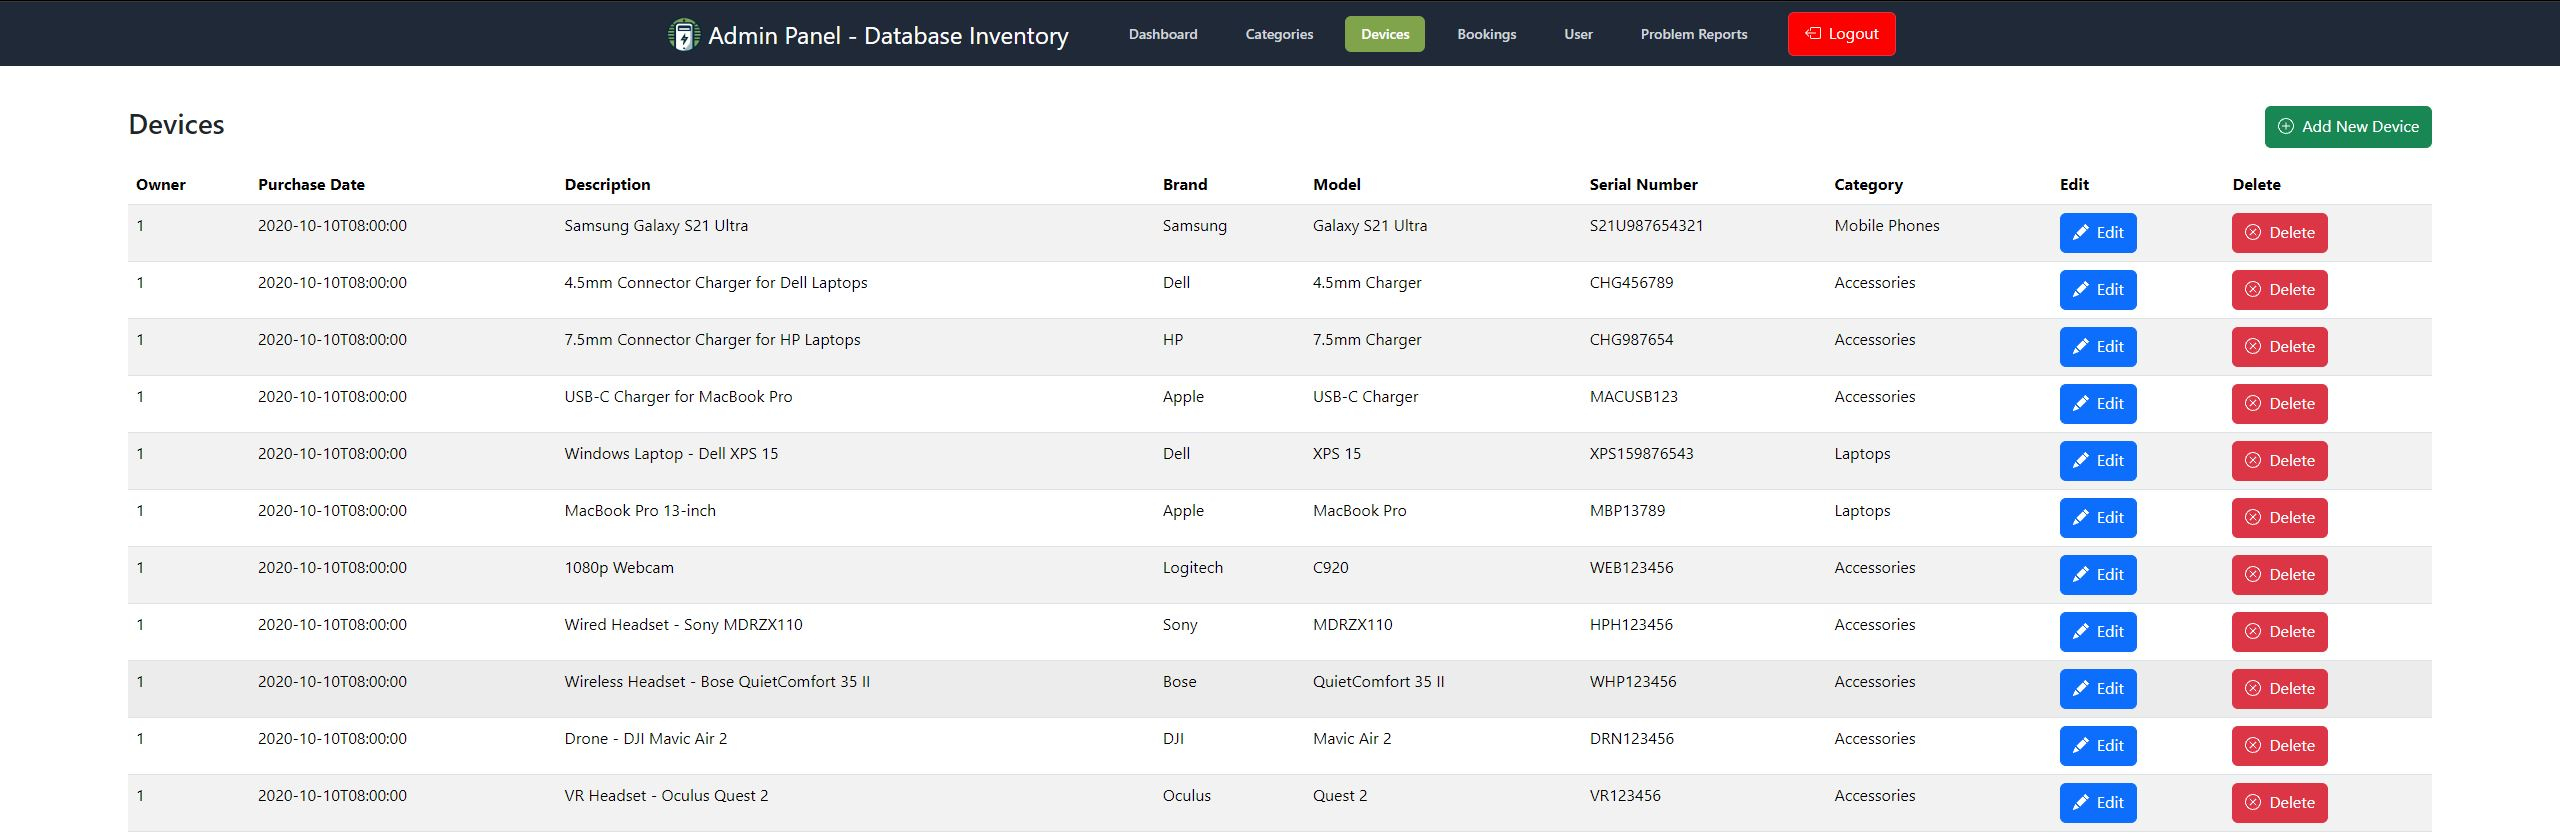
\includegraphics[width=1\linewidth]{images/devices.JPG}
    \caption{Admin Dashboard Devices}
    \label{fig:devices-dashboard}
\end{figure}

\item \textbf {Problem Reports Screen: }At the Problem Reports screen, administrators can review all user-submitted reports. Each report includes a photograph and is linked to the booking it pertains to, allowing for efficient and effective issue tracking and resolution.
\begin{figure}[h]
    \centering
    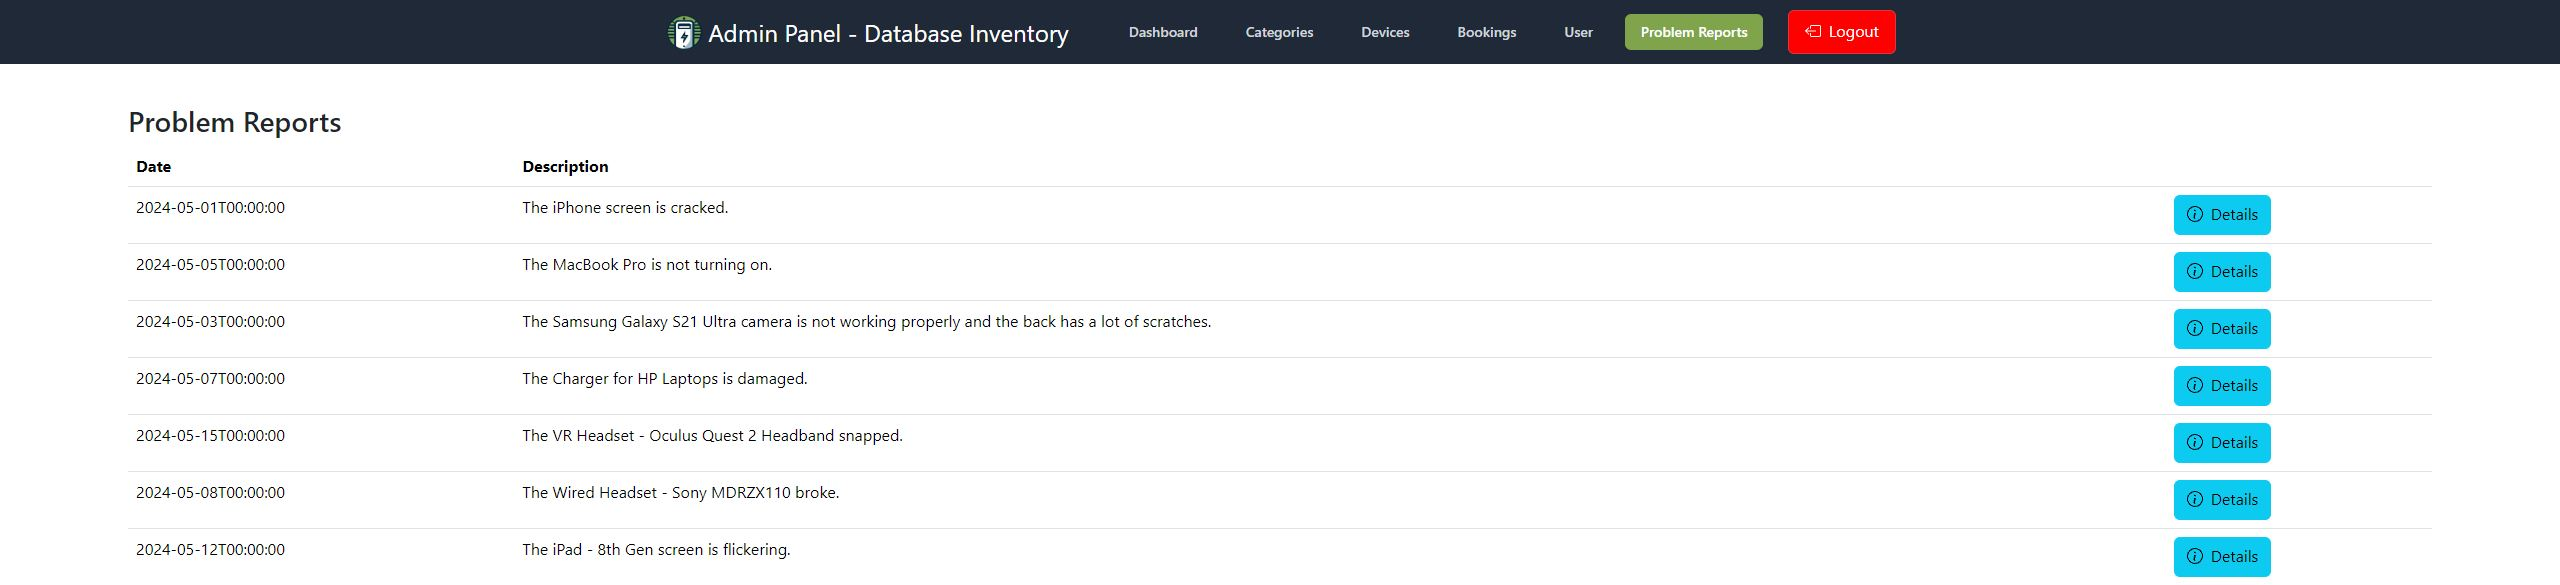
\includegraphics[width=1\linewidth]{images/problem reports.JPG}
    \caption{Admin Dashboard Problem Reports}
    \label{fig:problem-reports-dashboard}
\end{figure}
\newpage
\item \textbf{User Frontend Bookings: } This interface allows users to view all their bookings. It provides detailed information for each booking, including price, start and end times. Users can also terminate an ongoing booking directly from this screen. Additionally, for lockers rented for charging, a \textit{wattage} button is available to monitor power usage.
\begin{figure}[h]
    \centering
    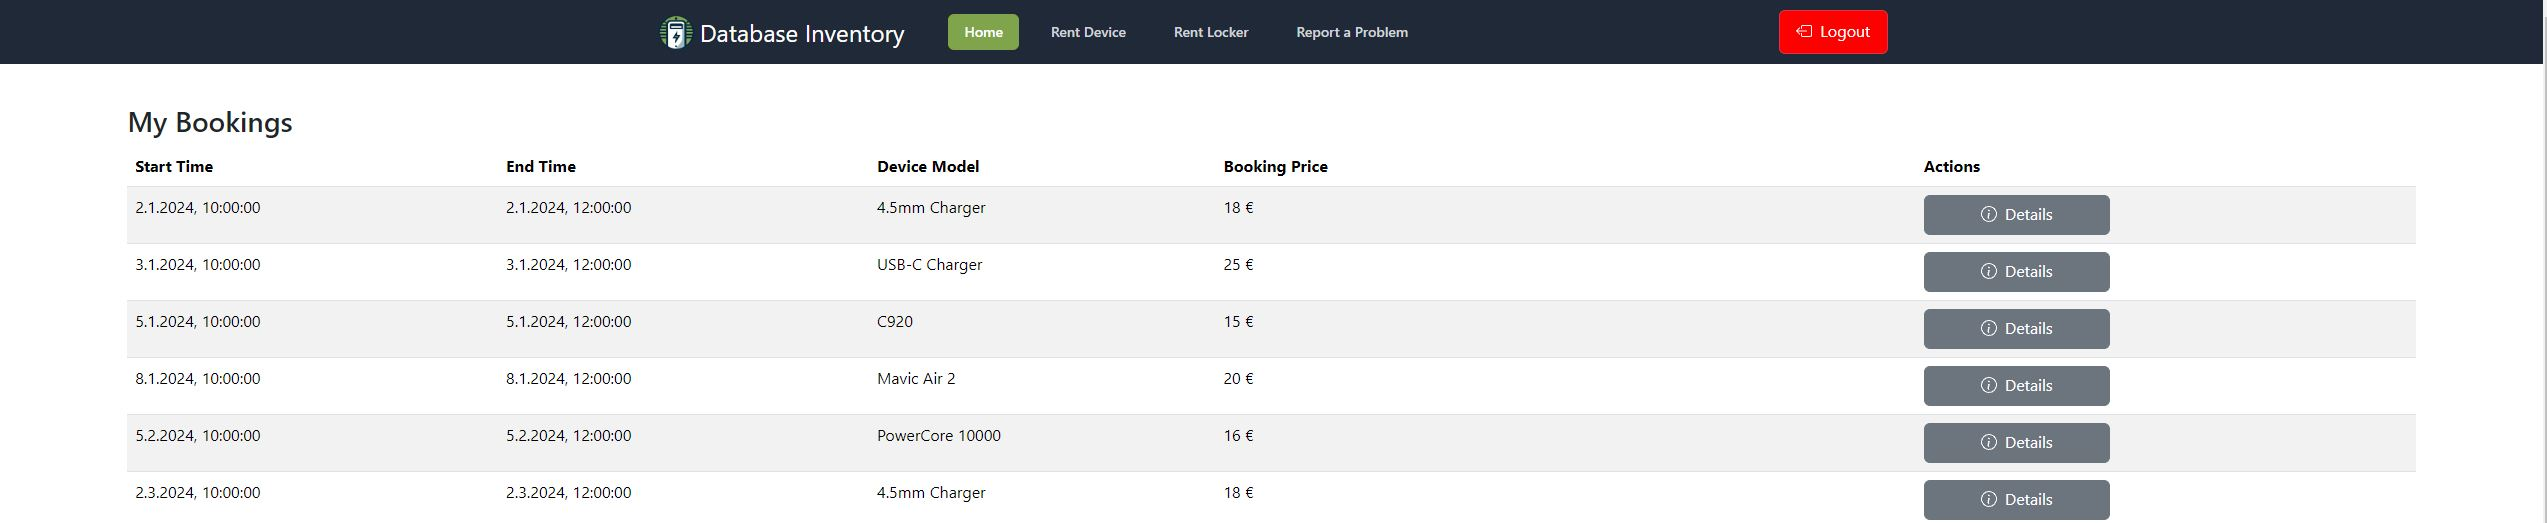
\includegraphics[width=1\linewidth]{images/bookings.JPG}
    \caption{User Frontend Bookings}
    \label{fig:user-bookings-dashboard}
\end{figure}

\item \textbf{User Frontend Rent Device: } This screen displays all available devices for rent, detailing the cost per hour and providing comprehensive information about each device. Users can select devices based on their specific needs and availability.
\begin{figure}[h]
    \centering
    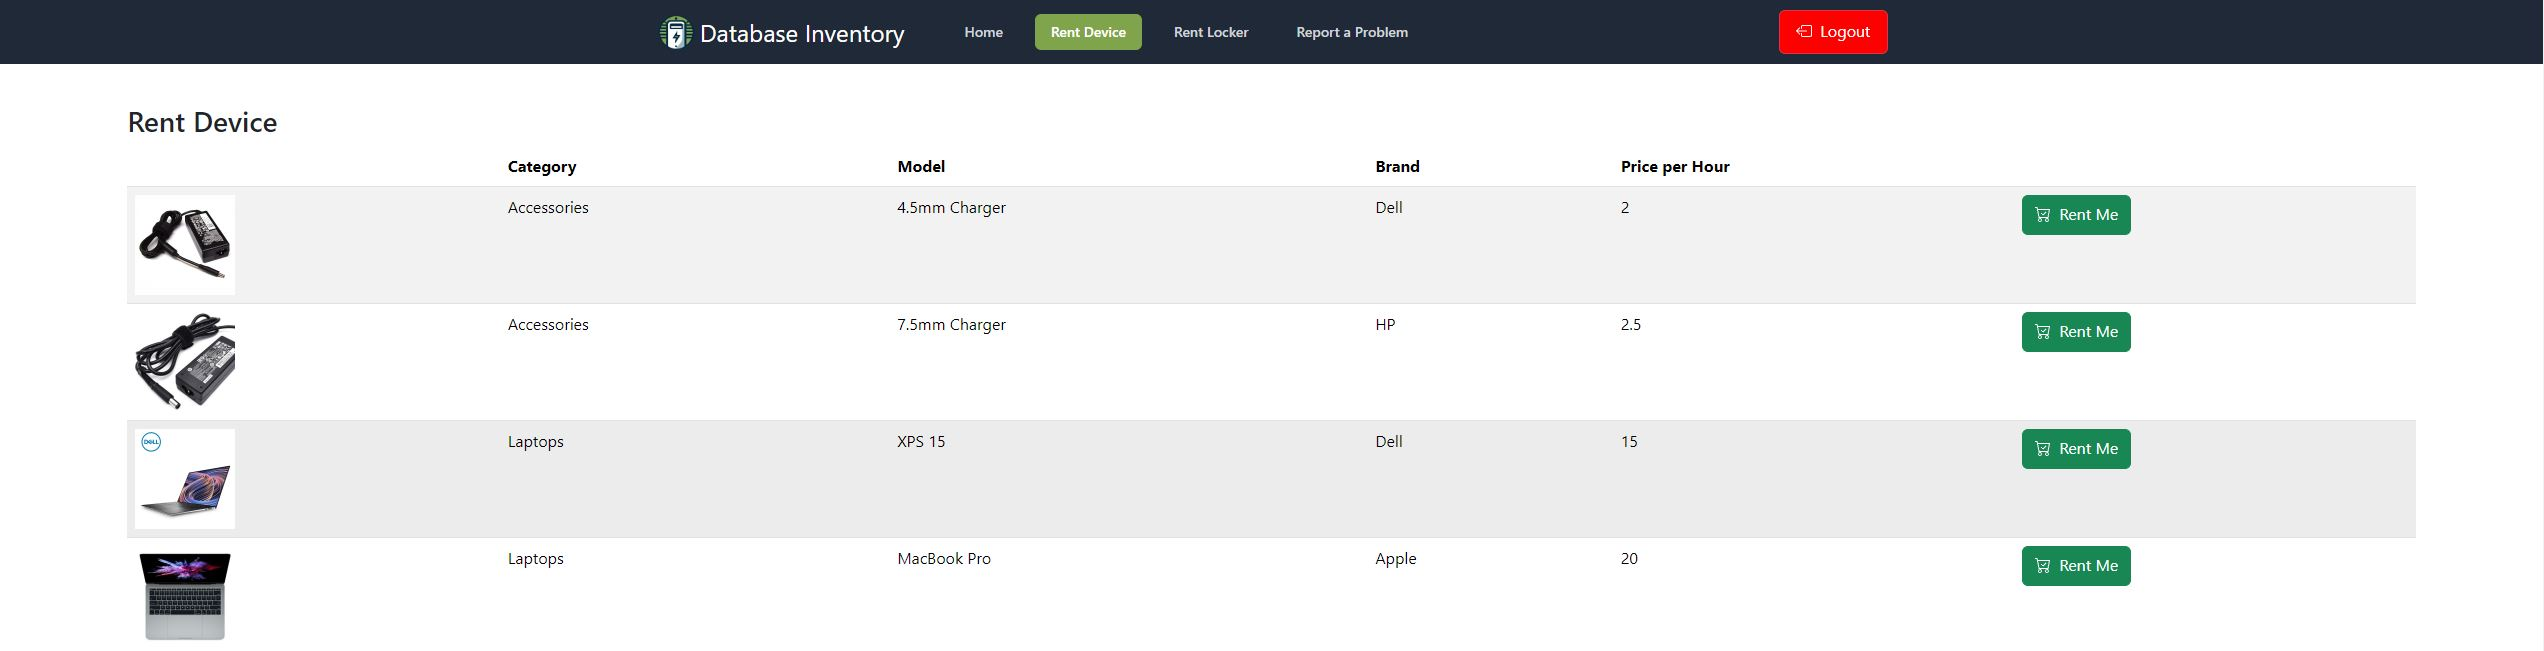
\includegraphics[width=1\linewidth]{images/rent device.JPG}
    \caption{User Frontend Rent Device}
    \label{fig:rent-device-dashboard}
\end{figure}
\newpage
\item \textbf{User Frontend Rent Device Confirmation: } In this confirmation modal, users receive a pin code to access the locker. Additionally, the modal includes a Google Map showing the location of the device or locker, enhancing user convenience.
\begin{figure}[h]
    \centering
    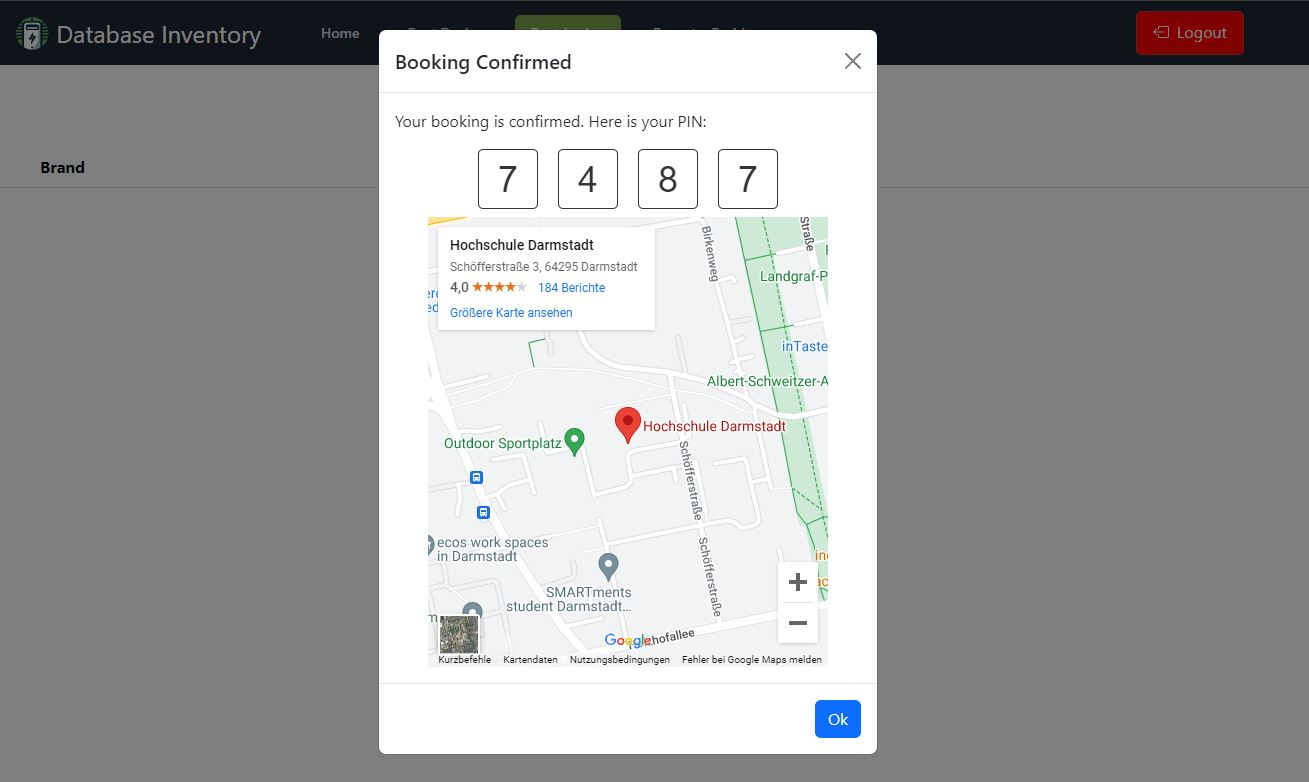
\includegraphics[width=1\linewidth]{images/booking conf.JPG}
    \caption{User Frontend Rent Device Confirmation}
    \label{fig:rent-device-confirmation-modal}
\end{figure}

\item \textbf{User Frontend Locker Wattage Overview: }This view provides users with real-time information on whether the device is currently charging. If the wattage flow is off, it indicates that the device is fully charged, offering users insight into the device's charging status.
\begin{figure}[h]
    \centering
    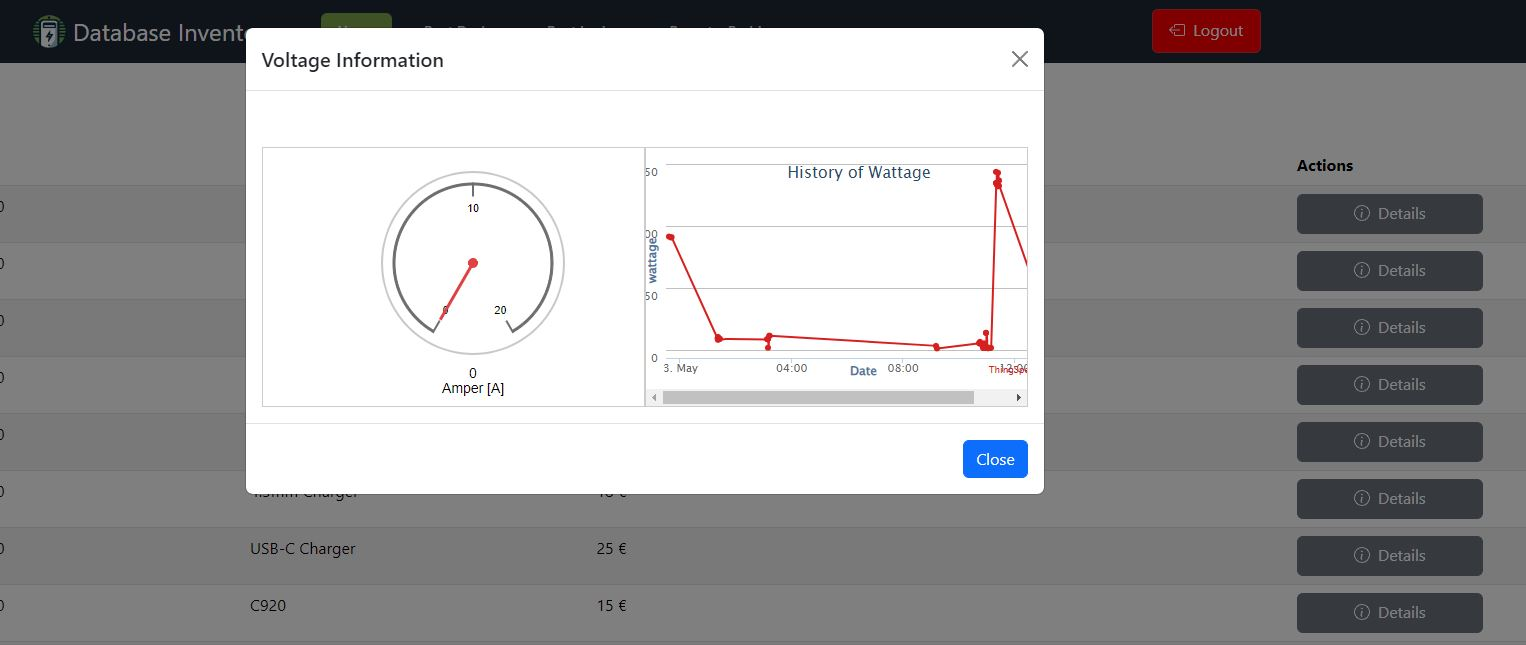
\includegraphics[width=1\linewidth]{images/user_wattage.JPG}
    \caption{User Frontend Locker Wattage Overview}
    \label{fig:locker-wattage-overview}
\end{figure}
\end{itemize}

